% Control loop figure for the A1 poster. Compile on its own, then in the poster:
%   \includegraphics[width=\linewidth]{images/fig_loop_poster.pdf}
\documentclass[12pt, border=4pt]{standalone}
\usepackage{tikz}
\usetikzlibrary{arrows.meta,positioning,calc,fit,backgrounds}
\renewcommand{\familydefault}{\sfdefault}

% poster theme colours
\definecolor{saclaydk}{RGB}{27,67,32}
\definecolor{mandarine}{RGB}{243,115,32}
\definecolor{vert}{RGB}{140,198,62}
\definecolor{bleu}{RGB}{80,144,205}
\definecolor{rouge}{RGB}{198,11,70}

\tikzset{
  box/.style={rounded corners=4pt, line width=1.4pt, align=center,
              text width=3.1cm, minimum height=2.4cm, inner sep=5pt},
  hw/.style={box, draw=saclaydk, fill=vert!18},
  data/.style={box, draw=bleu, fill=bleu!12},
  nn/.style={box, draw=mandarine, fill=mandarine!18, line width=2pt},
  arr/.style={-{Stealth[length=4mm,width=3mm]}, line width=2pt, draw=saclaydk!80},
  arrnn/.style={arr, draw=mandarine},
  ttl/.style={font=\large\bfseries},
}

\begin{document}
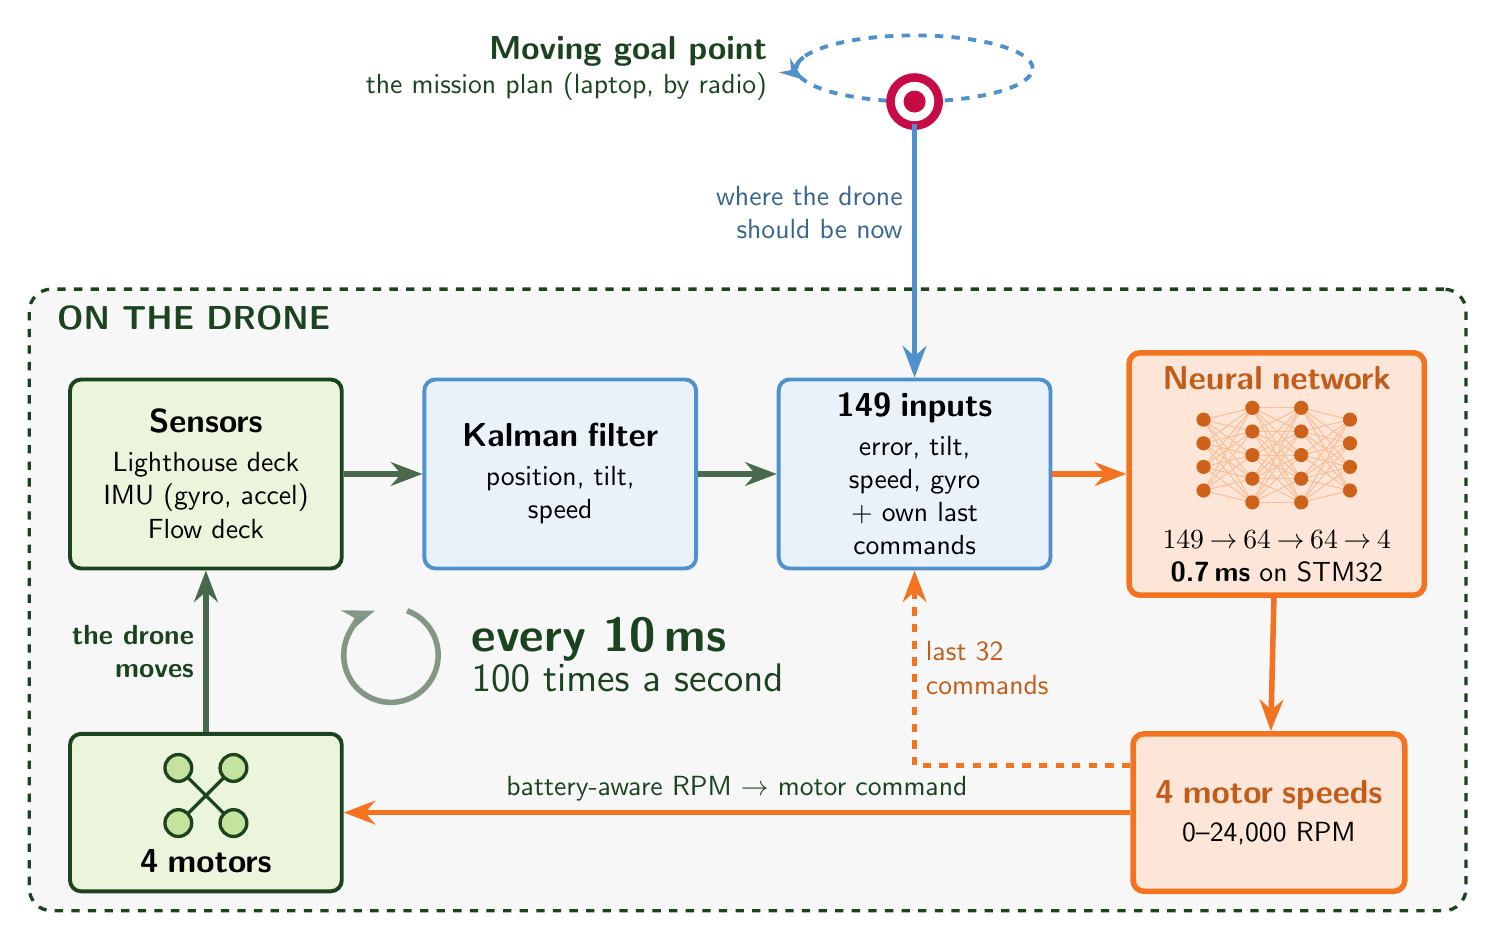
\begin{tikzpicture}
  % top row: sensing -> deciding
  \node[hw]   (sens) at (0,0)    {{\large\bfseries Sensors}\\[2pt]Lighthouse deck\\IMU (gyro, accel)\\Flow deck};
  \node[data] (kal)  at (4.5,0)  {{\large\bfseries Kalman filter}\\[2pt]position, tilt,\\speed};
  \node[data] (inp)  at (9,0)    {{\large\bfseries 149 inputs}\\[2pt]error, tilt,\\speed, gyro\\+ own last commands};
  \node[nn, text width=3.4cm]   (net)  at (13.6,0) {{\large\bfseries\color{mandarine!80!black} Neural network}\\[3pt]%
      \tikz[x=0.62cm, y=0.3cm]{%
        \foreach \a/\na in {0/4,1/5,2/5,3/4}{\foreach \b in {1,...,\na}{\coordinate (n\a-\b) at (\a, {(\na+1)/2-\b});}}
        \foreach \a/\na/\nb in {0/4/5,1/5/5,2/5/4}{\pgfmathtruncatemacro{\c}{\a+1}
          \foreach \i in {1,...,\na}{\foreach \j in {1,...,\nb}{\draw[mandarine!45, line width=0.4pt] (n\a-\i) -- (n\c-\j);}}}
        \foreach \a/\na in {0/4,1/5,2/5,3/4}{\foreach \b in {1,...,\na}{\fill[mandarine!85!black] (n\a-\b) circle (0.09cm);}}}\\[2pt]
      {\normalsize $149\!\to\!64\!\to\!64\!\to\!4$}\\\textbf{0.7\,ms} on STM32};

  % bottom row: acting
  \node[nn, minimum height=2cm]  (spd) at (13.5,-4.3) {{\large\bfseries\color{mandarine!80!black} 4 motor speeds}\\[2pt]0--24{,}000 RPM};
  \node[hw, minimum height=2cm]  (mot) at (0,-4.3) {%
      \tikz[baseline=-0.5ex, line width=1.2pt, saclaydk]{%
        \draw (-0.35,-0.35) -- (0.35,0.35) (-0.35,0.35) -- (0.35,-0.35);
        \foreach \x/\y in {-0.35/-0.35, 0.35/0.35, -0.35/0.35, 0.35/-0.35}
          \draw[fill=vert!50] (\x,\y) circle (0.17);}\\[3pt]
      {\large\bfseries 4 motors}};

  % main loop arrows
  \draw[arr]   (sens) -- (kal);
  \draw[arr]   (kal)  -- (inp);
  \draw[arrnn] (inp)  -- (net);
  \draw[arrnn] (net)  -- (spd);
  \draw[arrnn] (spd.west) -- node[above, font=\normalsize, text=saclaydk] {battery-aware RPM $\to$ motor command} (mot.east);
  \draw[arr]   (mot) -- node[left, font=\normalsize\bfseries, text=saclaydk, align=right] {the drone\\moves} (sens);

  % the network's own commands feed back into its inputs
  \draw[arrnn, dashed, line width=1.6pt] ($(spd.west)+(0,0.6)$) -| node[pos=0.75, right, font=\normalsize, text=mandarine!80!black, align=left] {last 32\\commands} (inp.south);

  % loop rate in the middle
  \draw[-{Stealth[length=4mm,width=3mm]}, line width=2pt, saclaydk!55] (2.35,-2.3) ++(70:0.6) arc[start angle=70, end angle=-250, radius=0.6];
  \node[anchor=west, align=left, text=saclaydk] at (3.25,-2.3) {{\LARGE\bfseries every 10\,ms}\\{\Large 100 times a second}};

  % drone panel
  \begin{scope}[on background layer]
    \node[draw=saclaydk, dashed, line width=1.2pt, rounded corners=8pt, fill=saclaydk!4,
          fit=(sens)(net)(spd)(mot), inner xsep=14pt, inner ysep=14pt, yshift=8pt] (drone) {};
  \end{scope}
  \node[anchor=north west, font=\large\bfseries, text=saclaydk] at ($(drone.north west)+(0.25,-0.12)$)
       {ON THE DRONE};

  % the mission: a goal point moving along a path (sent from the laptop)
  \begin{scope}[shift={(9,5.15)}]
    \draw[bleu, line width=1.4pt, dash pattern=on 3pt off 3pt] (0,0) ellipse (1.5 and 0.42);
    \draw[-{Stealth[length=3mm]}, bleu, line width=1.4pt] (160:1.5 and 0.42) arc[start angle=160, end angle=200, x radius=1.5, y radius=0.42];
    \foreach \r/\c in {0.36/rouge, 0.25/white, 0.14/rouge} \fill[\c] (0,-0.42) circle (\r);
  \end{scope}
  \node[anchor=east, align=right, text=saclaydk] at (7.25,5.15)
       {{\large\bfseries Moving goal point}\\{\normalsize the mission plan (laptop, by radio)}};
  \draw[arr, draw=bleu] (9,4.45) -- node[left, font=\normalsize, text=bleu!70!black, align=right, pos=0.35] {where the drone\\should be now} (inp.north);
\end{tikzpicture}
\end{document}
